\documentclass[]{book}
\usepackage{lmodern}
\usepackage{amssymb,amsmath}
\usepackage{ifxetex,ifluatex}
\usepackage{fixltx2e} % provides \textsubscript
\ifnum 0\ifxetex 1\fi\ifluatex 1\fi=0 % if pdftex
  \usepackage[T1]{fontenc}
  \usepackage[utf8]{inputenc}
\else % if luatex or xelatex
  \ifxetex
    \usepackage{mathspec}
  \else
    \usepackage{fontspec}
  \fi
  \defaultfontfeatures{Ligatures=TeX,Scale=MatchLowercase}
  \newcommand{\euro}{€}
\fi
% use upquote if available, for straight quotes in verbatim environments
\IfFileExists{upquote.sty}{\usepackage{upquote}}{}
% use microtype if available
\IfFileExists{microtype.sty}{%
\usepackage{microtype}
\UseMicrotypeSet[protrusion]{basicmath} % disable protrusion for tt fonts
}{}
\usepackage[margin=1in]{geometry}
\usepackage{hyperref}
\PassOptionsToPackage{usenames,dvipsnames}{color} % color is loaded by hyperref
\hypersetup{unicode=true,
            pdftitle={Rustr Book},
            pdfborder={0 0 0},
            breaklinks=true}
\urlstyle{same}  % don't use monospace font for urls
\usepackage{natbib}
\bibliographystyle{apalike}
\usepackage{color}
\usepackage{fancyvrb}
\newcommand{\VerbBar}{|}
\newcommand{\VERB}{\Verb[commandchars=\\\{\}]}
\DefineVerbatimEnvironment{Highlighting}{Verbatim}{commandchars=\\\{\}}
% Add ',fontsize=\small' for more characters per line
\usepackage{framed}
\definecolor{shadecolor}{RGB}{248,248,248}
\newenvironment{Shaded}{\begin{snugshade}}{\end{snugshade}}
\newcommand{\KeywordTok}[1]{\textcolor[rgb]{0.13,0.29,0.53}{\textbf{{#1}}}}
\newcommand{\DataTypeTok}[1]{\textcolor[rgb]{0.13,0.29,0.53}{{#1}}}
\newcommand{\DecValTok}[1]{\textcolor[rgb]{0.00,0.00,0.81}{{#1}}}
\newcommand{\BaseNTok}[1]{\textcolor[rgb]{0.00,0.00,0.81}{{#1}}}
\newcommand{\FloatTok}[1]{\textcolor[rgb]{0.00,0.00,0.81}{{#1}}}
\newcommand{\ConstantTok}[1]{\textcolor[rgb]{0.00,0.00,0.00}{{#1}}}
\newcommand{\CharTok}[1]{\textcolor[rgb]{0.31,0.60,0.02}{{#1}}}
\newcommand{\SpecialCharTok}[1]{\textcolor[rgb]{0.00,0.00,0.00}{{#1}}}
\newcommand{\StringTok}[1]{\textcolor[rgb]{0.31,0.60,0.02}{{#1}}}
\newcommand{\VerbatimStringTok}[1]{\textcolor[rgb]{0.31,0.60,0.02}{{#1}}}
\newcommand{\SpecialStringTok}[1]{\textcolor[rgb]{0.31,0.60,0.02}{{#1}}}
\newcommand{\ImportTok}[1]{{#1}}
\newcommand{\CommentTok}[1]{\textcolor[rgb]{0.56,0.35,0.01}{\textit{{#1}}}}
\newcommand{\DocumentationTok}[1]{\textcolor[rgb]{0.56,0.35,0.01}{\textbf{\textit{{#1}}}}}
\newcommand{\AnnotationTok}[1]{\textcolor[rgb]{0.56,0.35,0.01}{\textbf{\textit{{#1}}}}}
\newcommand{\CommentVarTok}[1]{\textcolor[rgb]{0.56,0.35,0.01}{\textbf{\textit{{#1}}}}}
\newcommand{\OtherTok}[1]{\textcolor[rgb]{0.56,0.35,0.01}{{#1}}}
\newcommand{\FunctionTok}[1]{\textcolor[rgb]{0.00,0.00,0.00}{{#1}}}
\newcommand{\VariableTok}[1]{\textcolor[rgb]{0.00,0.00,0.00}{{#1}}}
\newcommand{\ControlFlowTok}[1]{\textcolor[rgb]{0.13,0.29,0.53}{\textbf{{#1}}}}
\newcommand{\OperatorTok}[1]{\textcolor[rgb]{0.81,0.36,0.00}{\textbf{{#1}}}}
\newcommand{\BuiltInTok}[1]{{#1}}
\newcommand{\ExtensionTok}[1]{{#1}}
\newcommand{\PreprocessorTok}[1]{\textcolor[rgb]{0.56,0.35,0.01}{\textit{{#1}}}}
\newcommand{\AttributeTok}[1]{\textcolor[rgb]{0.77,0.63,0.00}{{#1}}}
\newcommand{\RegionMarkerTok}[1]{{#1}}
\newcommand{\InformationTok}[1]{\textcolor[rgb]{0.56,0.35,0.01}{\textbf{\textit{{#1}}}}}
\newcommand{\WarningTok}[1]{\textcolor[rgb]{0.56,0.35,0.01}{\textbf{\textit{{#1}}}}}
\newcommand{\AlertTok}[1]{\textcolor[rgb]{0.94,0.16,0.16}{{#1}}}
\newcommand{\ErrorTok}[1]{\textcolor[rgb]{0.64,0.00,0.00}{\textbf{{#1}}}}
\newcommand{\NormalTok}[1]{{#1}}
\usepackage{graphicx,grffile}
\makeatletter
\def\maxwidth{\ifdim\Gin@nat@width>\linewidth\linewidth\else\Gin@nat@width\fi}
\def\maxheight{\ifdim\Gin@nat@height>\textheight\textheight\else\Gin@nat@height\fi}
\makeatother
% Scale images if necessary, so that they will not overflow the page
% margins by default, and it is still possible to overwrite the defaults
% using explicit options in \includegraphics[width, height, ...]{}
\setkeys{Gin}{width=\maxwidth,height=\maxheight,keepaspectratio}
\setlength{\parindent}{0pt}
\setlength{\parskip}{6pt plus 2pt minus 1pt}
\setlength{\emergencystretch}{3em}  % prevent overfull lines
\providecommand{\tightlist}{%
  \setlength{\itemsep}{0pt}\setlength{\parskip}{0pt}}
\setcounter{secnumdepth}{5}

%%% Use protect on footnotes to avoid problems with footnotes in titles
\let\rmarkdownfootnote\footnote%
\def\footnote{\protect\rmarkdownfootnote}

%%% Change title format to be more compact
\usepackage{titling}

% Create subtitle command for use in maketitle
\newcommand{\subtitle}[1]{
  \posttitle{
    \begin{center}\large#1\end{center}
    }
}

\setlength{\droptitle}{-2em}
  \title{Rustr Book}
  \pretitle{\vspace{\droptitle}\centering\huge}
  \posttitle{\par}
  \author{}
  \preauthor{}\postauthor{}
  \predate{\centering\large\emph}
  \postdate{\par}
  \date{updated on 2016-04-24}


\usepackage{booktabs}
\usepackage{longtable}
\usepackage{framed,color}
\definecolor{shadecolor}{RGB}{248,248,248}

\ifxetex
  \usepackage{letltxmacro}
  \setlength{\XeTeXLinkMargin}{1pt}
  \LetLtxMacro\SavedIncludeGraphics\includegraphics
  \def\includegraphics#1#{% #1 catches optional stuff (star/opt. arg.)
    \IncludeGraphicsAux{#1}%
  }%
  \newcommand*{\IncludeGraphicsAux}[2]{%
    \XeTeXLinkBox{%
      \SavedIncludeGraphics#1{#2}%
    }%
  }%
\fi

\newenvironment{rmdblock}[1]
  {\begin{shaded*}
  \begin{itemize}
  \renewcommand{\labelitemi}{
    \raisebox{-.7\height}[0pt][0pt]{
      {\setkeys{Gin}{width=3em,keepaspectratio}\includegraphics{images/#1}}
    }
  }
  \item
  }
  {
  \end{itemize}
  \end{shaded*}
  }
\newenvironment{rmdnote}
  {\begin{rmdblock}{note}}
  {\end{rmdblock}}
\newenvironment{rmdcaution}
  {\begin{rmdblock}{caution}}
  {\end{rmdblock}}
\newenvironment{rmdimportant}
  {\begin{rmdblock}{important}}
  {\end{rmdblock}}
\newenvironment{rmdtip}
  {\begin{rmdblock}{tip}}
  {\end{rmdblock}}
\newenvironment{rmdwarning}
  {\begin{rmdblock}{warning}}
  {\end{rmdblock}}

% Redefines (sub)paragraphs to behave more like sections
\ifx\paragraph\undefined\else
\let\oldparagraph\paragraph
\renewcommand{\paragraph}[1]{\oldparagraph{#1}\mbox{}}
\fi
\ifx\subparagraph\undefined\else
\let\oldsubparagraph\subparagraph
\renewcommand{\subparagraph}[1]{\oldsubparagraph{#1}\mbox{}}
\fi

\begin{document}
\maketitle

{
\setcounter{tocdepth}{1}
\tableofcontents
}
\chapter{Introduction}\label{introduction}

\textbf{Rust and R Integration}

\texttt{rustr} is a Rust library that provides a Rust API to work with
R.

Write pure Rust code with \texttt{rustr}, and then use \texttt{rustinr}
R package to generate Rust interfaces to R.

This project is now under construction. Issues and Pull requests are
welcome!

\chapter{Setup}\label{setup}

Rustr support Linux, Mac, and Windows.

\begin{figure}[htbp]
\centering

\includegraphics{./images/setup.jpg}
\caption{Fuse Ring}
\end{figure}

\href{https://www.flickr.com/photos/fncll/8604144457/in/photolist-xELx44-aeGtnt-xbcPF1-nT2ZFk-o2wrom-xbcZxW-xs1Le9-xELyLn-xsQof6-mL9ndW-59oVCm-2wPrE-ec7aPH-wvX6sc-8pgKJf-9KiRJr-e7juoe-rzsGcV-7oofH7-2wPrn-dVsH5X-hLf6aW-66S3Qg-8G1fuT-2wPrt}{@
Chris Lott}
\href{https://creativecommons.org/licenses/by/2.0/deed.en}{CC 2.0}

\section{Windows}\label{windows}

\subsection{Get R}\label{get-r}

Get
\href{https://cran.r-project.org/bin/windows/base/R-3.3.0beta-win.exe}{R
\textgreater{} 3.3.0} builded by GCC 4.9 and
\href{https://cran.r-project.org/bin/windows/Rtools/Rtools33.exe}{Rtools
3.3}

\subsection{Get Rust with GNU ABI}\label{get-rust-with-gnu-abi}

Checkout \url{https://www.rust-lang.org/downloads.html}

One of stable, beta, or nightly version of Rust is OK. You can put Rust
installation in \texttt{PATH} or set \texttt{CARGO\_HOME} environment
variable to the path of \texttt{cargo.exe}.

If you want to build multi-arch R package, make sure you install both
64bit and 32bit Rust standard library, for example
\texttt{C:\textbackslash{}Rust\textbackslash{}lib\textbackslash{}rustlib\textbackslash{}i686-pc-windows-gnu}
and
\texttt{C:\textbackslash{}Rust\textbackslash{}lib\textbackslash{}rustlib\textbackslash{}x86\_64-pc-windows-gnu}

\subsection{Get rustinr}\label{get-rustinr}

Run This in R:

\begin{Shaded}
\begin{Highlighting}[]
\KeywordTok{install.packages}\NormalTok{(}\StringTok{"devtools"}\NormalTok{)}
\NormalTok{devtools::}\KeywordTok{install_github}\NormalTok{(}\StringTok{"rustr/rustinr"}\NormalTok{)}
\end{Highlighting}
\end{Shaded}

And we are ready to play!

Run this in R console.

\begin{Shaded}
\begin{Highlighting}[]
\KeywordTok{library}\NormalTok{(rustinr)}

\KeywordTok{rust}\NormalTok{(}\DataTypeTok{code =}\StringTok{'}
\StringTok{// #[rustr_export]}
\StringTok{pub fn say_hi() -> String\{}
\StringTok{    "Hello World".into()}
\StringTok{\}}
\StringTok{'}\NormalTok{)}

\KeywordTok{say_hi}\NormalTok{()}
\CommentTok{#> [1] "Hello World"}
\end{Highlighting}
\end{Shaded}

If some errors show up, run \texttt{check\_rustr} to get more info:

\begin{Shaded}
\begin{Highlighting}[]
\KeywordTok{check_rustr}\NormalTok{(}\DataTypeTok{detail =} \NormalTok{T)}
\end{Highlighting}
\end{Shaded}

\section{Mac}\label{mac}

\subsection{Get R}\label{get-r-1}

Get \href{https://cran.r-project.org/bin/macosx/}{R \textgreater{}
3.3.0}.

\subsection{Get Rust with GNU ABI}\label{get-rust-with-gnu-abi-1}

Checkout \url{https://www.rust-lang.org/downloads.html}

\begin{verbatim}
curl -sSf https://static.rust-lang.org/rustup.sh | sh
\end{verbatim}

One of Stable, Beta, or Nightly version of Rust is OK.

You can put Rust installation in path or set \texttt{CARGO\_HOME}
environment variable to the path of \texttt{cargo}.

\subsection{Get rustinr}\label{get-rustinr-1}

Run This in R:

\begin{Shaded}
\begin{Highlighting}[]
\KeywordTok{install.packages}\NormalTok{(}\StringTok{"devtools"}\NormalTok{)}
\NormalTok{devtools::}\KeywordTok{install_github}\NormalTok{(}\StringTok{"rustr/rustinr"}\NormalTok{)}
\end{Highlighting}
\end{Shaded}

\subsection{Get Xcode Command Line
Tools}\label{get-xcode-command-line-tools}

Open Terminal, and run \texttt{git} or \texttt{clang}, It may show a
message to get you started.

Or you can check
\href{http://rud.is/b/2015/10/20/installing-r-on-os-x/}{this great
guide}.

And we are ready to play!

Run this in R console.

\begin{Shaded}
\begin{Highlighting}[]
\KeywordTok{library}\NormalTok{(rustinr)}

\KeywordTok{rust}\NormalTok{(}\DataTypeTok{code =}\StringTok{'}
\StringTok{// #[rustr_export]}
\StringTok{pub fn say_hi() -> String\{}
\StringTok{    "Hello World".into()}
\StringTok{\}}
\StringTok{'}\NormalTok{)}

\KeywordTok{say_hi}\NormalTok{()}
\CommentTok{#> [1] "Hello World"}
\end{Highlighting}
\end{Shaded}

If some errors show up, run \texttt{check\_rustr} to get more info:

\begin{Shaded}
\begin{Highlighting}[]
\KeywordTok{check_rustr}\NormalTok{(}\DataTypeTok{detail =} \NormalTok{T)}
\end{Highlighting}
\end{Shaded}

\section{Linux}\label{linux}

\subsection{Get R}\label{get-r-2}

Get \href{https://cran.r-project.org/}{R \textgreater{} 3.3.0}.

\subsection{Get Rust with GNU ABI}\label{get-rust-with-gnu-abi-2}

\begin{Shaded}
\begin{Highlighting}[]
\KeywordTok{curl} \NormalTok{-sSf https://static.rust-lang.org/rustup.sh }\KeywordTok{|} \KeywordTok{sh}
\end{Highlighting}
\end{Shaded}

One of Stable, Beta, or Nightly version of Rust is OK.

You can put Rust installation in path or set \texttt{CARGO\_HOME}
environment variable to the path of \texttt{cargo}.

\subsection{Get rustinr}\label{get-rustinr-2}

Run This in R:

\begin{Shaded}
\begin{Highlighting}[]
\KeywordTok{install.packages}\NormalTok{(}\StringTok{"devtools"}\NormalTok{)}
\NormalTok{devtools::}\KeywordTok{install_github}\NormalTok{(}\StringTok{"rustr/rustinr"}\NormalTok{)}
\end{Highlighting}
\end{Shaded}

And we are ready to play!

Run this in R console.

\begin{Shaded}
\begin{Highlighting}[]
\KeywordTok{library}\NormalTok{(rustinr)}

\KeywordTok{rust}\NormalTok{(}\StringTok{'}
\StringTok{// #[rustr_export]}
\StringTok{pub fn say_hi() -> String\{}
\StringTok{    "Hello World".into()}
\StringTok{\}}
\StringTok{'}\NormalTok{)}

\KeywordTok{say_hi}\NormalTok{()}
\CommentTok{#> [1] "Hello World"}
\end{Highlighting}
\end{Shaded}

If some errors show up, run \texttt{check\_rustr} to get more info:

\begin{Shaded}
\begin{Highlighting}[]
\KeywordTok{check_rustr}\NormalTok{(}\DataTypeTok{detail =} \NormalTok{T)}
\end{Highlighting}
\end{Shaded}

\section{Playground with Docker}\label{playground-with-docker}

Visit \url{https://play.rustr.org} , and begin to code Rust in R.

This Web App is run in a Docker container. If you want to run this app
locally. You can install
\href{https://docs.docker.com/windows/}{Docker}, and then run:

\begin{Shaded}
\begin{Highlighting}[]
\KeywordTok{docker} \NormalTok{pull qinwf/shiny-rust-docker}

\KeywordTok{docker} \NormalTok{run -p 3838:3838 qinwf/shiny-rust-docker}
\end{Highlighting}
\end{Shaded}

Visit \url{http://127.0.0.1:3838} for your local version of rustr
playground.

You can also run this Docker image with an R console that supports Rust:

\begin{Shaded}
\begin{Highlighting}[]
\KeywordTok{docker} \NormalTok{run -ti --rm qinwf/shiny-rust-docker R}
\end{Highlighting}
\end{Shaded}

\chapter{Run}\label{run}

Now we will begin to code Rust in R.

\begin{figure}[htbp]
\centering
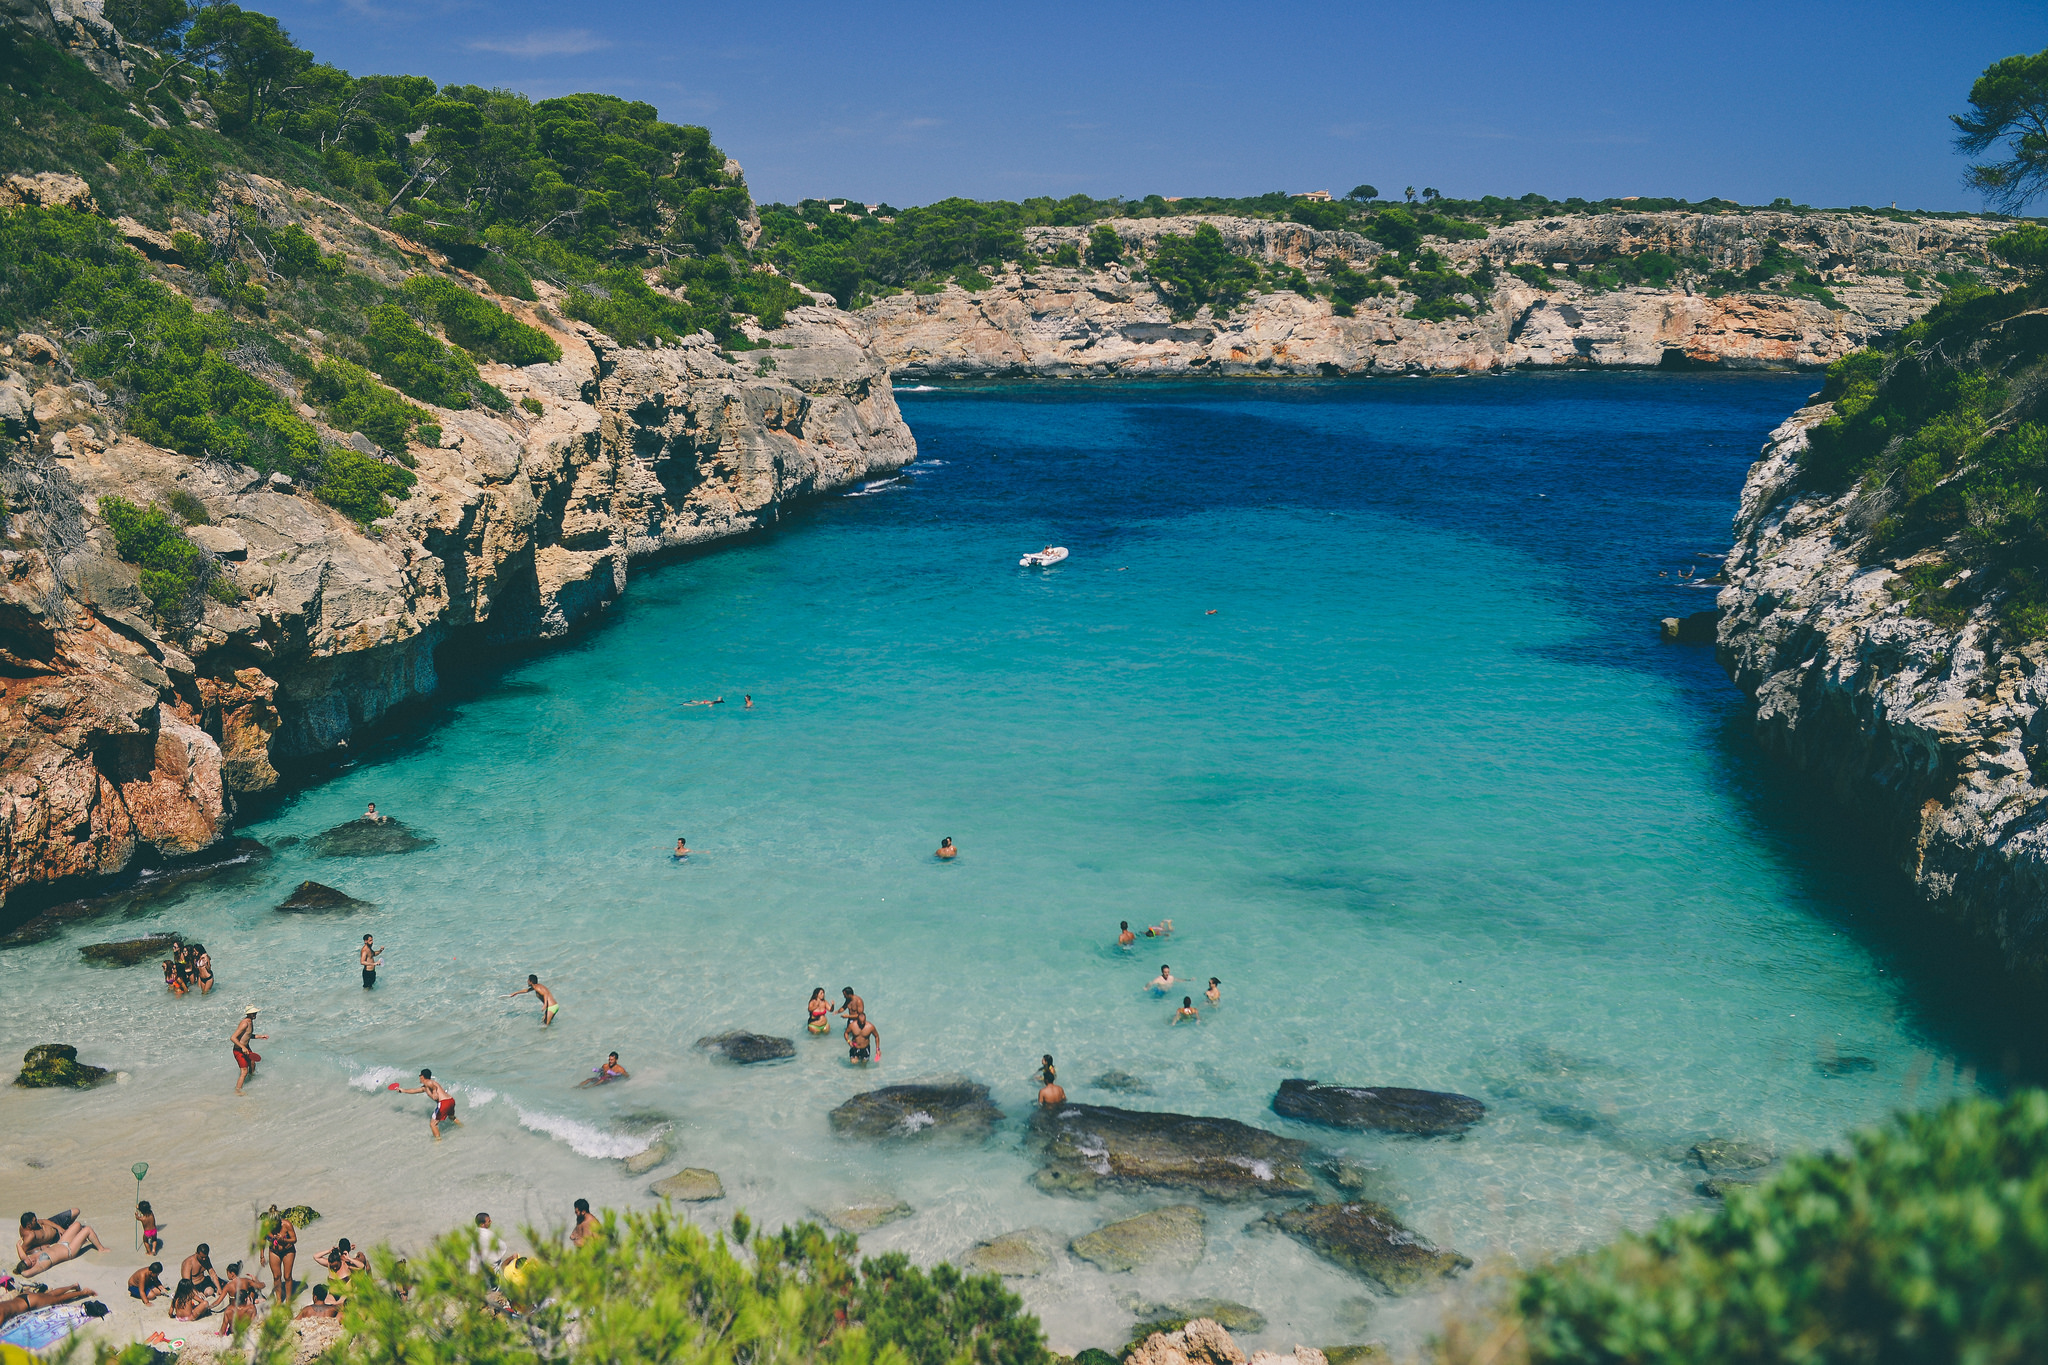
\includegraphics{./images/run.jpg}
\caption{Dive In}
\end{figure}

\href{https://www.flickr.com/photos/nathancongleton/10002041966/}{@
Nathan Congleton}
\href{https://creativecommons.org/licenses/by-nc-sa/2.0/}{CC BY-NC-SA
2.0}

\section{\texorpdfstring{\texttt{rustinr} R
package}{rustinr R package}}\label{rustinr-r-package}

\texttt{rustinr} is a R package to help user generate the basic struture
of a Rust-R package and source Rust script in R. Install it with

\begin{Shaded}
\begin{Highlighting}[]
\NormalTok{devtools::}\KeywordTok{install_github}\NormalTok{(}\StringTok{"rustr/rustinr"}\NormalTok{)}
\end{Highlighting}
\end{Shaded}

\subsection{Rust Function in R
Console}\label{rust-function-in-r-console}

\texttt{rust()} is a R function to create Rust function in R console
interatively.

For a Rust function:

\begin{Shaded}
\begin{Highlighting}[]
\KeywordTok{pub} \KeywordTok{fn} \NormalTok{say_hi() -> }\DataTypeTok{String}\NormalTok{\{}
    \StringTok{"Hello World"}\NormalTok{.into()}
\NormalTok{\}}
\end{Highlighting}
\end{Shaded}

Just mark it with \texttt{//\ \#{[}rustr\_export{]}}, and put this
function in \texttt{rust()}

\begin{Shaded}
\begin{Highlighting}[]
\KeywordTok{library}\NormalTok{(rustinr)}

\KeywordTok{rust}\NormalTok{(}\DataTypeTok{code =} \StringTok{'}
\StringTok{// #[rustr_export]}
\StringTok{pub fn say_hi() -> String\{}
\StringTok{    "Hello World".into()}
\StringTok{\}}
\StringTok{'}\NormalTok{)}

\KeywordTok{say_hi}\NormalTok{()}
\CommentTok{#> [1] "Hello World"}
\end{Highlighting}
\end{Shaded}

and then you can call \texttt{say\_hi} in R.

\begin{Shaded}
\begin{Highlighting}[]
\NormalTok{say_hi}
\CommentTok{#> function () }
\CommentTok{#> \{}
\CommentTok{#>     .Call("ouNIkssJBKBM_say_hi", PACKAGE = "ouNIkssJBKBM")}
\CommentTok{#> \}}
\end{Highlighting}
\end{Shaded}

Here is another example:

\begin{Shaded}
\begin{Highlighting}[]
\KeywordTok{rust}\NormalTok{(}\DataTypeTok{code =} \StringTok{'}
\StringTok{// #[rustr_export]}
\StringTok{pub fn fib_rs(x:u64)-> u64\{}
\StringTok{    if x == 0 \{ return 0 \};}
\StringTok{    if x == 1 \{ return 1 \};}
\StringTok{    return fib_rs(x - 1) + fib_rs(x - 2);}
\StringTok{\}'}\NormalTok{)}

\KeywordTok{fib_rs}\NormalTok{(10L)}
\CommentTok{#> [1] 55}
\end{Highlighting}
\end{Shaded}

For more example, you can also checkout \url{https://gallery.rustr.org}

\section{Create a Rust-R Package}\label{create-a-rust-r-package}

\subsection{Init a Package}\label{init-a-package}

\texttt{rustr\_init} will create an R package with Rust support.

Just run:

\begin{Shaded}
\begin{Highlighting}[]
\KeywordTok{rustr_init}\NormalTok{(}\StringTok{"pkgname"}\NormalTok{,}\StringTok{"."}\NormalTok{)}
\CommentTok{#> Creating directories ...}
\CommentTok{#> Creating DESCRIPTION ...}
\CommentTok{#> Creating NAMESPACE ...}
\CommentTok{#> Creating Read-and-delete-me ...}
\CommentTok{#> Saving functions and data ...}
\CommentTok{#> Making help files ...}
\CommentTok{#> Done.}
\CommentTok{#> Further steps are described in './pkgname/Read-and-delete-me'.}
\CommentTok{#> added useDynLib to NAMESPACE}

\KeywordTok{list.dirs}\NormalTok{(}\StringTok{"pkgname"}\NormalTok{)}
\CommentTok{#> [1] "pkgname"                 "pkgname/man"            }
\CommentTok{#> [3] "pkgname/R"               "pkgname/src"            }
\CommentTok{#> [5] "pkgname/src/rustlib"     "pkgname/src/rustlib/src"}
\end{Highlighting}
\end{Shaded}

\texttt{pkgname/src/rustlib} is a Rust library, for more info see
\url{http://doc.crates.io/}

Rust files are in \texttt{pkgname/src/rustlib/src}.

\texttt{pkgname/src/rustlib/src/lib.rs} should begin with:

\begin{Shaded}
\begin{Highlighting}[]
\CommentTok{# Run This In R}
\KeywordTok{headr}\NormalTok{()}
\CommentTok{#> #[macro_use]}
\CommentTok{#> extern crate rustr;}
\CommentTok{#> pub mod export;}
\CommentTok{#> pub use rustr::*;}
\CommentTok{#> }
\CommentTok{#> // #[rustr_export]}
\CommentTok{#> pub fn say_hi()->RResult<String>\{}
\CommentTok{#>    Ok("hello world".into())}
\CommentTok{#> \}}
\end{Highlighting}
\end{Shaded}

or

\begin{Shaded}
\begin{Highlighting}[]
\AttributeTok{#[}\NormalTok{macro_use}\AttributeTok{]}
\KeywordTok{extern} \KeywordTok{crate} \NormalTok{rustr;}
\KeywordTok{pub} \KeywordTok{mod} \NormalTok{export;}
\KeywordTok{pub} \KeywordTok{use} \NormalTok{rustr::*;}
\end{Highlighting}
\end{Shaded}

\subsection{\texorpdfstring{Intro
\texttt{rustrize()}}{Intro rustrize()}}\label{intro-rustrize}

Rust function begin with \texttt{//\ \#{[}rustr\_export{]}} will be
imported to R by \texttt{rustrize()} R function.

\begin{Shaded}
\begin{Highlighting}[]
\CommentTok{// /src/rustlib/src/lib.rs}

\AttributeTok{#[}\NormalTok{macro_use}\AttributeTok{]}
\KeywordTok{extern} \KeywordTok{crate} \NormalTok{rustr;}
\KeywordTok{pub} \KeywordTok{mod} \NormalTok{export;}
\KeywordTok{pub} \KeywordTok{use} \NormalTok{rustr::*;}

\CommentTok{// ' Roxygen Comment Header (Optional)}
\CommentTok{// ' }
\CommentTok{// ' detail info about function}
\CommentTok{// ' @param a parameter detail}
\CommentTok{// ' @export}
\CommentTok{// #[rustr_export]}
\KeywordTok{pub} \KeywordTok{fn} \NormalTok{say_hi()-> }\DataTypeTok{String}\NormalTok{\{}
    \StringTok{"Hello World!"}\NormalTok{.into()}
\NormalTok{\}}
\end{Highlighting}
\end{Shaded}

and then run \texttt{rustrize()}.

\subsubsection{Generated Files}\label{generated-files}

These files are generated by \texttt{rustrize()}.

\begin{enumerate}
\def\labelenumi{\arabic{enumi}.}
\tightlist
\item
  \texttt{/R/REXPORT.R} - \texttt{.Call()} binding in R.
\item
  \texttt{/src/REXPORT.c} - Exported \texttt{.Call()} Functions.
\item
  \texttt{/src/rustlib/src/export.rs} - A public module in
  /src/rustlib/src/lib.rs, this module export Rust function to R.
\end{enumerate}

\begin{Shaded}
\begin{Highlighting}[]
\CommentTok{# /R/REXPORT.R}

\CommentTok{#' Roxygen Comment Header (Optional)}
\CommentTok{#' }
\CommentTok{#' detail info about function}
\CommentTok{#' @param a parameter detail}
\CommentTok{#' @export}
\NormalTok{say_hi =}\StringTok{ }\NormalTok{function()\{ }\KeywordTok{.Call}\NormalTok{(}\StringTok{'SvhCRFYxjsuH_say_hi'}\NormalTok{,}\DataTypeTok{PACKAGE =} \StringTok{'SvhCRFYxjsuH'}\NormalTok{)\}}
\end{Highlighting}
\end{Shaded}

\begin{Shaded}
\begin{Highlighting}[]
\CommentTok{// /src/REXPORT.c}

\OtherTok{#include <Rinternals.h>}
\OtherTok{#include <R.h>}

\KeywordTok{extern} \NormalTok{SEXP rustr_say_hi();}
\NormalTok{SEXP SvhCRFYxjsuH_say_hi()\{ }\KeywordTok{return}\NormalTok{(rustr_say_hi());\}}
\end{Highlighting}
\end{Shaded}

\begin{Shaded}
\begin{Highlighting}[]
\CommentTok{// /src/rustlib/src/export.rs}

\KeywordTok{use} \KeywordTok{super}\NormalTok{::*;}

\AttributeTok{#[}\NormalTok{no_mangle}\AttributeTok{]}
\KeywordTok{pub} \KeywordTok{extern} \StringTok{"C"} \KeywordTok{fn} \NormalTok{rustr_say_hi()->SEXP\{}

 \KeywordTok{let} \NormalTok{res  = say_hi();}

 \KeywordTok{let} \NormalTok{res_sexp : SEXP = }\PreprocessorTok{unwrapr!}\NormalTok{(res.intor());}

 \KeywordTok{return} \NormalTok{res_sexp;}
\NormalTok{\}}
\end{Highlighting}
\end{Shaded}

And your R package are ready to \texttt{R\ CMD\ build}.

\section{Summary}\label{summary}

\subsection{rust()}\label{rust}

\begin{Shaded}
\begin{Highlighting}[]
\KeywordTok{rust}\NormalTok{(}\DataTypeTok{path =} \StringTok{"Rust file"}\NormalTok{, }\DataTypeTok{code =} \StringTok{"Rust code"}\NormalTok{, }\DataTypeTok{depend =} \StringTok{"Optional Cargo TOML dependency"}\NormalTok{)}
\end{Highlighting}
\end{Shaded}

Source Rust file or code in R console.

\subsection{rustr\_init()}\label{rustrux5finit}

\begin{Shaded}
\begin{Highlighting}[]
\KeywordTok{rustr_init}\NormalTok{(}\DataTypeTok{name =} \StringTok{"R package name"}\NormalTok{, }\DataTypeTok{path =} \StringTok{"Pacakage path"}\NormalTok{)}
\end{Highlighting}
\end{Shaded}

Init a Rust-R package struture. It is similar to
\texttt{package.skeleton()}.

\subsection{headr()}\label{headr}

\begin{Shaded}
\begin{Highlighting}[]
\KeywordTok{headr}\NormalTok{()}
\end{Highlighting}
\end{Shaded}

Give you the header of the \texttt{lib.rs} for Rust Library to get
started with R.

\subsection{rustrize()}\label{rustrize}

\begin{Shaded}
\begin{Highlighting}[]
\KeywordTok{rustrize}\NormalTok{(}\DataTypeTok{path =} \StringTok{"."}\NormalTok{)}
\end{Highlighting}
\end{Shaded}

Generate R function for Rust function in a R package. It is similar to
\texttt{compileAttributes()} in \texttt{Rcpp}.

\chapter{Rusty Error Handling}\label{rusty-error-handling}

\subsection{RResult}\label{rresult}

Do you want to \texttt{Throw} \texttt{Throw} \texttt{Throw}?? Sorry You
can not!

But you can \texttt{try!()} \texttt{try!()} or \texttt{rtry!()}.

Make sure you learn enough Rust and read the
\href{https://doc.rust-lang.org/book/error-handling.html}{Rust Book}

This is \texttt{Monadic\ Error\ Handling}. If you do not know what it
means, just forget it. It is not that kind of bad \_ss thing.

If a Rust function may cause error, and need to throw a exception in R,
you can return RResult as your function return type.

For example,

\begin{Shaded}
\begin{Highlighting}[]
\KeywordTok{pub} \KeywordTok{fn} \NormalTok{rinteger(x : SEXP)->RResult<}\DataTypeTok{usize}\NormalTok{>\{}
    \KeywordTok{let} \NormalTok{res :RResult<}\DataTypeTok{usize}\NormalTok{> = }\DataTypeTok{usize}\NormalTok{::rnew(x);}
    \NormalTok{res}
\NormalTok{\}}
\end{Highlighting}
\end{Shaded}

Trait \texttt{RNew} will convert \texttt{SEXP} R Object Pointer to Rust
type. It may fail, so it return
\texttt{RResult\textless{}some\_type\textgreater{}}.

\begin{Shaded}
\begin{Highlighting}[]
\KeywordTok{rust}\NormalTok{(}\DataTypeTok{code =} \StringTok{'}
\StringTok{// #[rustr_export]}
\StringTok{pub fn rinteger(x : SEXP)->RResult<usize>\{}
\StringTok{    let res :RResult<usize> = usize::rnew(x);}
\StringTok{    res}
\StringTok{\}}
\StringTok{'}\NormalTok{)}

\KeywordTok{rinteger}\NormalTok{(}\DecValTok{1}\NormalTok{)}
\CommentTok{#> Error in eval(expr, envir, enclos): NotCompatible: expecting a integer}

\KeywordTok{rinteger}\NormalTok{(1L)}
\CommentTok{#> [1] 1}

\NormalTok{e =}\StringTok{ }\KeywordTok{tryCatch}\NormalTok{(}\KeywordTok{rinteger}\NormalTok{(}\DecValTok{1}\NormalTok{), }\DataTypeTok{error =} \NormalTok{function(e) e)}
\NormalTok{e}
\CommentTok{#> <NotCompatible in eval(expr, envir, enclos): NotCompatible: expecting a integer>}

\KeywordTok{str}\NormalTok{(e)}
\CommentTok{#> List of 2}
\CommentTok{#>  $ message: chr "NotCompatible: expecting a integer"}
\CommentTok{#>  $ call   : language eval(expr, envir, enclos)}
\CommentTok{#>  - attr(*, "class")= chr [1:4] "NotCompatible" "RustError" "error" "condition"}
\end{Highlighting}
\end{Shaded}

\chapter{R Console Print in Rust}\label{r-console-print-in-rust}

There are several ways to print to R console.

\subsection{\texorpdfstring{\texttt{r\_printf()}}{r\_printf()}}\label{rux5fprintf}

Print messages.

\begin{Shaded}
\begin{Highlighting}[]
\NormalTok{r_printf(&}\PreprocessorTok{format!}\NormalTok{(}\StringTok{"\{\}, \{\}, \{\}"}\NormalTok{, }\StringTok{"1"}\NormalTok{, }\DecValTok{2}\NormalTok{, }\DecValTok{3}\NormalTok{))}
\end{Highlighting}
\end{Shaded}

\subsection{\texorpdfstring{\texttt{r\_message()}}{r\_message()}}\label{rux5fmessage}

Print messages, which can be suppressed.

\begin{Shaded}
\begin{Highlighting}[]
\NormalTok{r_message(}\StringTok{"bing!"}\NormalTok{)}
\end{Highlighting}
\end{Shaded}

\subsection{\texorpdfstring{\texttt{r\_warn()}}{r\_warn()}}\label{rux5fwarn}

Print warnings.

\begin{Shaded}
\begin{Highlighting}[]
\NormalTok{r_warn(}\StringTok{"warning!"}\NormalTok{)}
\end{Highlighting}
\end{Shaded}

\subsection{\texorpdfstring{\texttt{rprint()}}{rprint()}}\label{rprint}

Print R Objects.

\begin{Shaded}
\begin{Highlighting}[]
\KeywordTok{let} \NormalTok{res : NumVec = }\PreprocessorTok{try!}\NormalTok{(NumVec::rnew(x))}
\NormalTok{rprint(res)}
\end{Highlighting}
\end{Shaded}

\chapter{R Type \textless{}-\textgreater{} Rust
Type}\label{r-type---rust-type}

Let's look at the code generated by rustrize().

\subsection{Origin:}\label{origin}

\begin{Shaded}
\begin{Highlighting}[]
\KeywordTok{pub} \KeywordTok{fn} \NormalTok{say_hi(a:}\DataTypeTok{String}\NormalTok{)-> }\DataTypeTok{String}\NormalTok{\{}
    \NormalTok{a}
\NormalTok{\}}
\end{Highlighting}
\end{Shaded}

\subsection{Generated:}\label{generated}

\begin{Shaded}
\begin{Highlighting}[]
\AttributeTok{#[}\NormalTok{no_mangle}\AttributeTok{]}
\KeywordTok{pub} \KeywordTok{extern} \StringTok{"C"} \KeywordTok{fn} \NormalTok{rustr_say_hi(a : SEXP)->SEXP\{}

 \KeywordTok{let} \NormalTok{a_ : }\DataTypeTok{String} \NormalTok{= }\PreprocessorTok{unwrapr!}\NormalTok{( }\DataTypeTok{String}\NormalTok{::rnew(a) );}
 \KeywordTok{let} \NormalTok{res  = say_hi(a_);}

 \KeywordTok{let} \NormalTok{res_sexp : SEXP = }\PreprocessorTok{unwrapr!}\NormalTok{(res.intor());}

 \KeywordTok{return} \NormalTok{res_sexp;}
\NormalTok{\}}
\end{Highlighting}
\end{Shaded}

\texttt{rustr\_say\_hi} takes a SEXP R pointer and then uses
\texttt{String::rnew} to convert SEXP to Rust String.

\subsection{RNew}\label{rnew}

\texttt{rnew} is from trait \texttt{RNew}:

\begin{Shaded}
\begin{Highlighting}[]
\KeywordTok{pub} \KeywordTok{trait} \NormalTok{RNew }\KeywordTok{where} \KeywordTok{Self}\NormalTok{: }\BuiltInTok{Sized}
\NormalTok{\{}
    \KeywordTok{fn} \NormalTok{rnew(x: SEXP) -> RResult<}\KeywordTok{Self}\NormalTok{>;}
\NormalTok{\}}
\end{Highlighting}
\end{Shaded}

\texttt{String} impl \texttt{RNew}, so we can call
\texttt{String::rnew(SEXP)}.

\begin{Shaded}
\begin{Highlighting}[]
\KeywordTok{impl} \NormalTok{RNew }\KeywordTok{for} \DataTypeTok{String} \NormalTok{\{}
    \KeywordTok{fn} \NormalTok{rnew(x: SEXP) -> RResult<}\DataTypeTok{String}\NormalTok{> \{}
        \NormalTok{.....}
    \NormalTok{\}}
\NormalTok{\}}
\end{Highlighting}
\end{Shaded}

And that is all. If you want to use you \textbf{own} awesome Rust type
as input for R function. impl \texttt{RNew} for it.

\subsection{IntoR}\label{intor}

\begin{Shaded}
\begin{Highlighting}[]
\AttributeTok{#[}\NormalTok{no_mangle}\AttributeTok{]}
\KeywordTok{pub} \KeywordTok{extern} \StringTok{"C"} \KeywordTok{fn} \NormalTok{rustr_say_hi(a : SEXP)->SEXP\{}

 \KeywordTok{let} \NormalTok{a_ : }\DataTypeTok{String} \NormalTok{= }\PreprocessorTok{unwrapr!}\NormalTok{( }\DataTypeTok{String}\NormalTok{::rnew(a) );}
 \KeywordTok{let} \NormalTok{res  = say_hi(a_);}

 \KeywordTok{let} \NormalTok{res_sexp : SEXP = }\PreprocessorTok{unwrapr!}\NormalTok{(res.intor());}

 \KeywordTok{return} \NormalTok{res_sexp;}
\NormalTok{\}}
\end{Highlighting}
\end{Shaded}

From \texttt{say\_hi(a\_)} we get a \texttt{String}, and then we run
\texttt{res.intor()}. \texttt{String} impl \texttt{IntoR}, so we can
call \texttt{res.intor()}.

\begin{Shaded}
\begin{Highlighting}[]
\KeywordTok{pub} \KeywordTok{trait} \NormalTok{IntoR \{}
    \KeywordTok{fn} \NormalTok{intor(&}\KeywordTok{self}\NormalTok{) -> RResult<SEXP>;}
\NormalTok{\}}
\end{Highlighting}
\end{Shaded}

\texttt{RNew} - R type to a new Rust type

\texttt{IntoR} - Rust type to R type

Hope this is simple enough.

If you want to use you \textbf{own} awesome Rust type as
\textbf{output}. impl \texttt{IntoR} for it.

\subsection{Orphan Rule}\label{orphan-rule}

There is an orphan rule to take care. Only your \textbf{own} Rust type
can impl traits from \texttt{rustr} crates.

If you want to impl \texttt{RNew} for
\texttt{Vec\textless{}String\textgreater{}}, you may not get lucky. But
you can create a struct to wrap Vec. Zero-cost abstraction feature of
Rust often helps you eliminate the overhead.

\subsection{\texorpdfstring{\texttt{RNew} \texttt{IntoR} impl Added to
\texttt{rustr}
Crate?}{RNew IntoR impl Added to rustr Crate?}}\label{rnew-intor-impl-added-to-rustr-crate}

Create a pull request!

We will consider support some rust crates with feature tag. For example,
\href{https://github.com/lifthrasiir/rust-chrono}{\texttt{chrono}} crate
for time.

\chapter{Type Table}\label{type-table}

There are many types!

\begin{figure}[htbp]
\centering

\includegraphics{./images/bridge.jpg}
\caption{Bridge}
\end{figure}

\href{https://www.flickr.com/photos/kitkit201/16133394909/in/photostream/}{@
Gloria Garcia}
\href{https://creativecommons.org/licenses/by-nc-nd/2.0/}{CC BY-NC-ND
2.0}

\section{R and Rust Type}\label{r-and-rust-type}

\subsection{R type}\label{r-type}

SEXP pointer in R has these types:

\begin{Shaded}
\begin{Highlighting}[]
\KeywordTok{typedef} \KeywordTok{enum} \NormalTok{\{}
    \NormalTok{NILSXP  = }\DecValTok{0}\NormalTok{,    }\CommentTok{/* nil = NULL */}
    \NormalTok{SYMSXP  = }\DecValTok{1}\NormalTok{,    }\CommentTok{/* symbols */}
    \NormalTok{LISTSXP = }\DecValTok{2}\NormalTok{,    }\CommentTok{/* lists of dotted pairs */}
    \NormalTok{CLOSXP  = }\DecValTok{3}\NormalTok{,    }\CommentTok{/* closures */}
    \NormalTok{ENVSXP  = }\DecValTok{4}\NormalTok{,    }\CommentTok{/* environments */}
    \NormalTok{PROMSXP = }\DecValTok{5}\NormalTok{,    }\CommentTok{/* promises: [un]evaluated closure arguments */}
    \NormalTok{LANGSXP = }\DecValTok{6}\NormalTok{,    }\CommentTok{/* language constructs (special lists) */}
    \NormalTok{SPECIALSXP  = }\DecValTok{7}\NormalTok{,    }\CommentTok{/* special forms */}
    \NormalTok{BUILTINSXP  = }\DecValTok{8}\NormalTok{,    }\CommentTok{/* builtin non-special forms */}
    \NormalTok{CHARSXP = }\DecValTok{9}\NormalTok{,    }\CommentTok{/* "scalar" string type (internal only)*/}
    \NormalTok{LGLSXP  = }\DecValTok{10}\NormalTok{,   }\CommentTok{/* logical vectors */}
    \NormalTok{INTSXP  = }\DecValTok{13}\NormalTok{,   }\CommentTok{/* integer vectors */}
    \NormalTok{REALSXP = }\DecValTok{14}\NormalTok{,   }\CommentTok{/* real variables */}
    \NormalTok{CPLXSXP = }\DecValTok{15}\NormalTok{,   }\CommentTok{/* complex variables */}
    \NormalTok{STRSXP  = }\DecValTok{16}\NormalTok{,   }\CommentTok{/* string vectors */}
    \NormalTok{DOTSXP  = }\DecValTok{17}\NormalTok{,   }\CommentTok{/* dot-dot-dot object */}
    \NormalTok{ANYSXP  = }\DecValTok{18}\NormalTok{,   }\CommentTok{/* make "any" args work */}
    \NormalTok{VECSXP  = }\DecValTok{19}\NormalTok{,   }\CommentTok{/* generic vectors */}
    \NormalTok{EXPRSXP = }\DecValTok{20}\NormalTok{,   }\CommentTok{/* expressions vectors */}
    \NormalTok{BCODESXP    = }\DecValTok{21}\NormalTok{,   }\CommentTok{/* byte code */}
    \NormalTok{EXTPTRSXP   = }\DecValTok{22}\NormalTok{,   }\CommentTok{/* external pointer */}
    \NormalTok{WEAKREFSXP  = }\DecValTok{23}\NormalTok{,   }\CommentTok{/* weak reference */}
    \NormalTok{RAWSXP  = }\DecValTok{24}\NormalTok{,   }\CommentTok{/* raw bytes */}
    \NormalTok{S4SXP   = }\DecValTok{25}\NormalTok{,   }\CommentTok{/* S4 non-vector */}

    \NormalTok{NEWSXP      = }\DecValTok{30}\NormalTok{,   }\CommentTok{/* fresh node creaed in new page */}
    \NormalTok{FREESXP     = }\DecValTok{31}\NormalTok{,   }\CommentTok{/* node released by GC */}

    \NormalTok{FUNSXP  = }\DecValTok{99}    \CommentTok{/* Closure or Builtin */}
\NormalTok{\} SEXPTYPE;}
\end{Highlighting}
\end{Shaded}

From R source code, see
\href{https://github.com/wch/r-source/blob/10617567bb97827f4b68b375e67f409f6013d93b/src/include/Rinternals.h\#L148-L178}{r-source}

\subsection{Rust type}\label{rust-type}

Rust standard container, such as \texttt{Vec} \texttt{LinkedList} are
all supported. And there are some other types are supported with feature
tags.

For example, DMat of \texttt{nalgebra} can be used with
\texttt{ty\_nalgebra} feature tag.

\section{The Type Table}\label{the-type-table}

You can also see
\href{http://docs.rustr.org/rustr/traits/trait.RNew.html}{Rust Docs} and
csv files on
\href{https://github.com/rustr/book/blob/master/type_table.csv}{GitHub}

\begin{tabular}{l|l|l|l|l|l}
\hline
Version & Traits & From & To & Feature & Remove.Version\\
\hline
0.1.5 & RNew URNew & LGLSXP & bool & default & NA\\
\hline
0.1.5 & RNew URNew & INTSXP & u64 & default & NA\\
\hline
0.1.5 & RNew URNew & INTSXP & u32 & default & NA\\
\hline
0.1.5 & RNew URNew & INTSXP & u16 & default & NA\\
\hline
0.1.5 & RNew URNew & INTSXP & i64 & default & NA\\
\hline
0.1.5 & RNew URNew & INTSXP & i32 & default & NA\\
\hline
0.1.5 & RNew URNew & INTSXP & i16 & default & NA\\
\hline
0.1.5 & RNew URNew & INTSXP & i8 & default & NA\\
\hline
0.1.5 & RNew URNew & INTSXP & usize & default & NA\\
\hline
0.1.5 & RNew URNew & INTSXP & isize & default & NA\\
\hline
0.1.5 & RNew URNew & REALSXP & f64 & default & NA\\
\hline
0.1.5 & RNew URNew & REALSXP & f32 & default & NA\\
\hline
0.1.5 & RNew URNew & INTSXP RAWSXP & u8 & default & NA\\
\hline
0.1.5 & RNew URNew & INTSXP & Vec<u64> & default & NA\\
\hline
0.1.5 & RNew URNew & INTSXP & Vec<u32> & default & NA\\
\hline
0.1.5 & RNew URNew & INTSXP & Vec<u16> & default & NA\\
\hline
0.1.5 & RNew URNew & INTSXP & Vec<i64> & default & NA\\
\hline
0.1.5 & RNew URNew & INTSXP & Vec<i32> & default & NA\\
\hline
0.1.5 & RNew URNew & INTSXP & Vec<i16> & default & NA\\
\hline
0.1.5 & RNew URNew & INTSXP & Vec<i8> & default & NA\\
\hline
\end{tabular}

\chapter{R Object}\label{r-object}

More in \href{https://docs.rustr.org/rustr/}{Rust Docs}.

\begin{figure}[htbp]
\centering
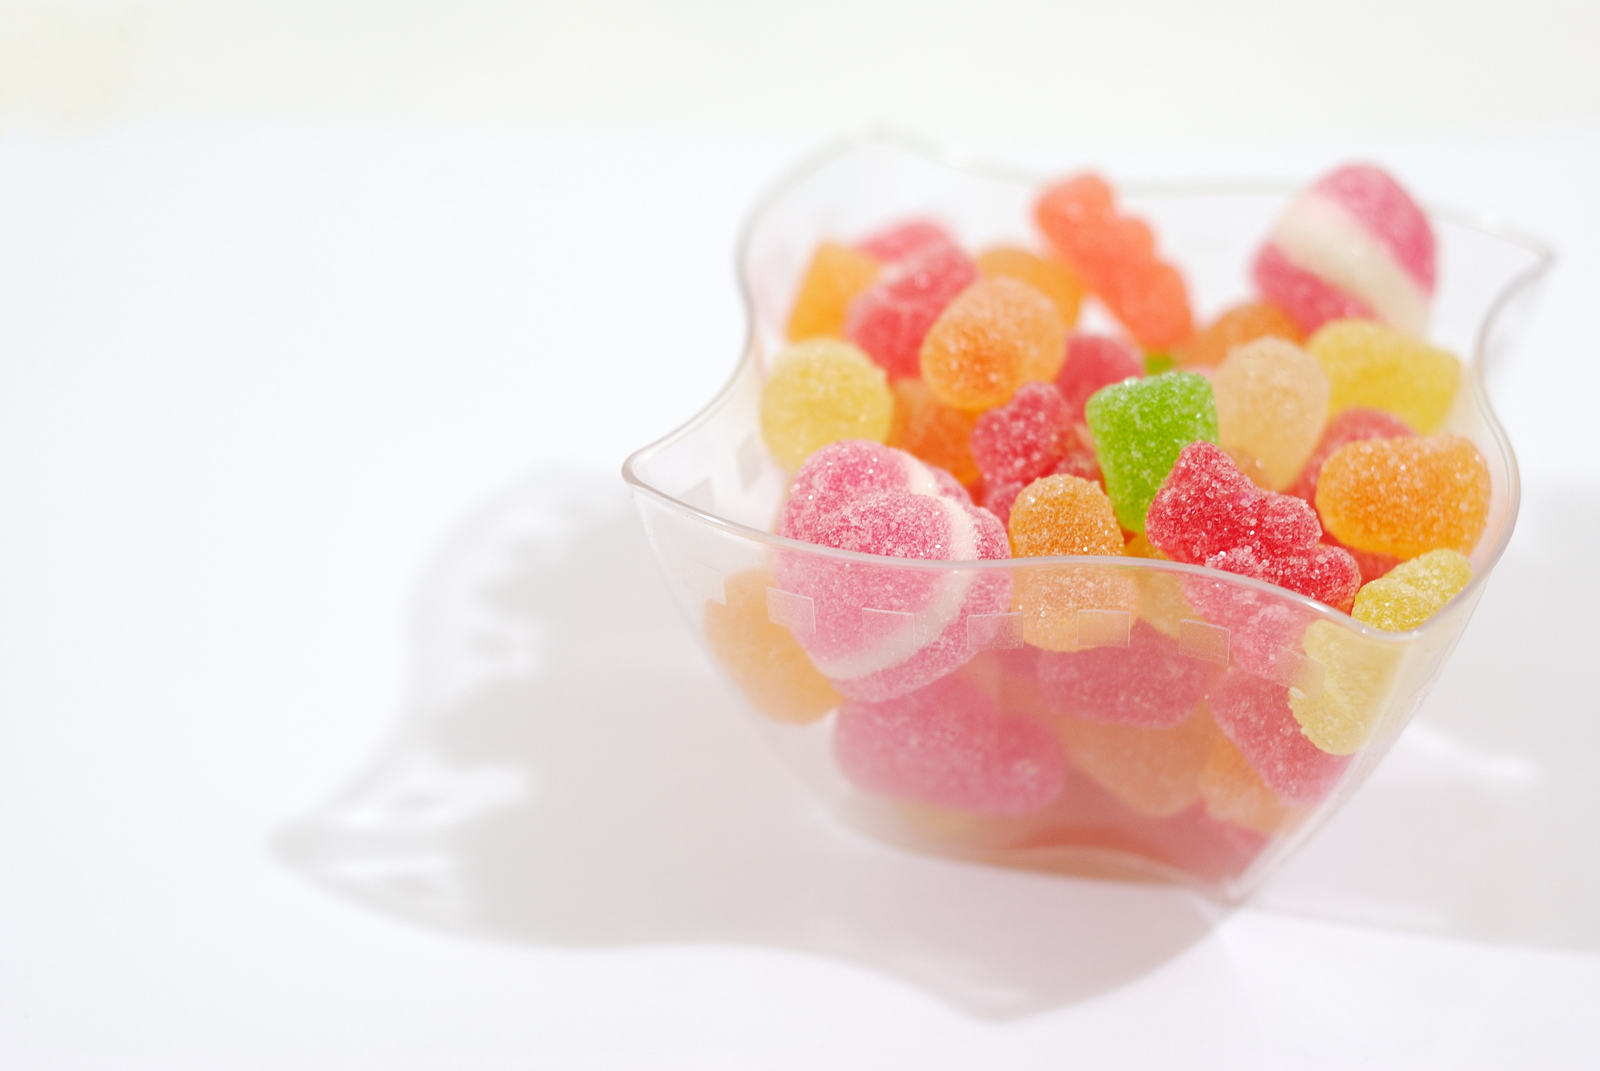
\includegraphics{./images/sugar.jpg}
\caption{Sweet}
\end{figure}

\href{https://www.flickr.com/photos/fl4y/5411655538/}{@ Gloria Garcia}
\href{https://creativecommons.org/licenses/by-nc-nd/2.0/}{CC BY-NC-ND
2.0}

\section{Vector}\label{vector}

TODO

\url{https://docs.rustr.org/rustr/vector/index.html}

\subsection{NumVec}\label{numvec}

\url{https://docs.rustr.org/rustr/vector/numvec/struct.NumVecM.html}

\subsection{IntVec}\label{intvec}

\url{https://docs.rustr.org/rustr/vector/intvec/struct.IntVecM.html}

\subsection{RawVec}\label{rawvec}

\url{https://docs.rustr.org/rustr/vector/rawvec/struct.RawVecM.html}

\subsection{BoolVec}\label{boolvec}

\url{https://docs.rustr.org/rustr/vector/boolvec/struct.BoolVecM.html}

\subsection{CplVec}\label{cplvec}

\url{https://docs.rustr.org/rustr/vector/cplvec/struct.CplVecM.html}

\section{VectorX - Special Vector}\label{vectorx---special-vector}

\subsection{CharVec}\label{charvec}

\url{https://docs.rustr.org/rustr/vectorx/charvec/struct.CharVecM.html}

\subsection{List}\label{list}

\url{https://docs.rustr.org/rustr/vectorx/list/struct.RListM.html}

\subsection{ExprVec}\label{exprvec}

\url{https://docs.rustr.org/rustr/vectorx/exprvec/struct.ExprVecM.html}

\section{Rcomplex}\label{rcomplex}

\url{https://docs.rustr.org/rustr/rdll/win64/struct.Struct_Unnamed9.html}

\section{Envir - Enviroment}\label{envir---enviroment}

\url{https://docs.rustr.org/rustr/environment/struct.EnvirM.html}

\section{RFun - Function}\label{rfun---function}

\url{https://docs.rustr.org/rustr/rfunction/struct.RFunM.html}

\section{RPtr - External Pointer}\label{rptr---external-pointer}

\url{https://docs.rustr.org/rustr/rptr/struct.RPtrM.html}

\section{Fml - Formula}\label{fml---formula}

\url{https://docs.rustr.org/rustr/formula/struct.RFmlM.html}

\section{RError - Error}\label{rerror---error}

\url{https://docs.rustr.org/rustr/error/struct.RError.html}

\section{Symbol - Symbol}\label{symbol---symbol}

\url{https://docs.rustr.org/rustr/symbol/struct.SymbolM.html}

\section{Promise - Promise}\label{promise---promise}

\url{https://docs.rustr.org/rustr/promise/struct.PromiseM.html}

\section{S4 - S4}\label{s4---s4}

\url{https://docs.rustr.org/rustr/s4/struct.S4M.html}

\section{Reference - RC}\label{reference---rc}

\url{https://docs.rustr.org/rustr/reference/struct.ReferenceM.html}

\section{RObj - Object}\label{robj---object}

\url{https://docs.rustr.org/rustr/robject/struct.RObjM.html}

\section{RWeak - Weak Reference}\label{rweak---weak-reference}

\url{https://docs.rustr.org/rustr/rweak/struct.RWeakM.html}

\section{RRand - Random Source}\label{rrand---random-source}

\url{https://docs.rustr.org/rustr/feature/random/struct.RRand.html}

\section{RLang - Language}\label{rlang---language}

\url{https://docs.rustr.org/rustr/rlang/struct.RLangM.html}

\chapter{\texorpdfstring{R Raw FFI with \texttt{unsafe}
Rust}{R Raw FFI with unsafe Rust}}\label{r-raw-ffi-with-unsafe-rust}

If you are interested in C API, you can read the docs about raw R-C API.

\url{https://docs.rustr.org/rustr/rdll/index.html} and
\url{https://docs.rustr.org/rustr/rdll/win64/index.html}

These APIs are generated by
\href{https://github.com/crabtw/rust-bindgen}{rust-bindgen}

\chapter{Cheat Sheet}\label{cheat-sheet}

\bibliography{book.bib}

\end{document}
